\documentclass{article}
\usepackage[left=2.50cm,right=2.50cm,top=2.50cm,bottom=2.50cm]{geometry}
\usepackage[pdftex]{graphicx}
\usepackage{amsmath, amssymb, hyperref}
\usepackage{float}
\usepackage{program}
\usepackage[all]{xy}

\begin{document}

\title{Solution to Homework-3}
\author{Sanath Kumar Ramesh, A50054305}
\date{20-April-2011}
\maketitle

\section{Problem-1}
\subsection{}
To find isotope profiles, one needs to construct a isotope abundance polynomial for each atom. Given a peptide, the number of atoms of each kind is computed. The isotope abundance polynomial for each atom in the peptide is multiplied to get an abundance polynomial for the whole peptide. The probability of the $i^{th}$ isotopic profile is given by the coefficient of $x^{i}$ in the polynomial for the peptide. 

This algorithm is already given in the lecture slides. They key part is to speedup the multiplication of polynomials. For this, I used Fast Fourier Transform. To multiply two polynomials $A(x)$ and $B(x)$ using FFT, the idea is as follows:

\begin{enumerate}
	\item Use FFT to evaluate $A(x)$ at each $x=\omega_{n}^{i}$ where $n$ is the degree-bound of $A(x)$, $\omega_{n}^{i}$ is the $i-th$ root of $\omega^{n}=1$ ie. $n^{th}$ root of unity.

	\item Similar to previous step, evaluate $B(x)$ with FFT.

	\item Take vector dot product of the output of above two steps ie. $ FFT( A(x) ) * FFT( B(x) )$ .

	\item Take inverse FFT of the result from above step - $FFT^{-1}(\ FFT( A(x) ) * FFT( B(x) )\ )$. The result gives the coefficients of each $x^{i}$ in the product of $A(x)$ and $B(x)$. This coefficient is what gives the isotopic profile.
\end{enumerate}

The program is written generically to accept any atoms, any amino acid and any abundance probability for each atom. Currently, it contains the abundance probability of C-12, C-13; H-1,H-2; N-14,N-15; O-16,O-18; S-32,S-33. The following results were generated with these profiles. Extending the program to take in other isotopes is a matter of adding some more entries in "input.h" file. This is very trivial. The "polynomial.h" file has the class that represents a polynomial and has the FFT routine in it which can help multiply two polynomials. To input different peptide to the program, the peptide's name is changed in the main() function.

The results for SLAMMER are as follows. Although the program will output all isotope profiles, I show here only the top ten. For comparison of  accuracy, I show the output obtained through ProteinProphet's \href{http://prospector.ucsf.edu/prospector/cgi-bin/msform.cgi?form=msisotope}{MS-Isotope tool}. The values in the table are percentages. The graph following the table shows the isotope profile for all isotopes as plotted with R. Since the values become very small, there is no visible difference between most points in the graph.

\ \\ \\ 

\begin{tabular}{|c|c|c|}
\hline
Isotope\# & ProteinProphet(\%) & Mytool(\%) \\ \hline
0 & 58.16 &	58.33 \\ \hline
1 & 25.31 &	28.06 \\ \hline
2 & 11.84 &	09.93 \\ \hline
3 & 3.51 &	2.57 \\ \hline
4 & 0.92 &	0.55 \\ \hline
5 & 0.2	  &   0.1 \\ \hline
6 & 0.04 &	0.02 \\ \hline
7 & 0.01 &	0.00 \\ \hline
8 & 0	& 0.00 \\ \hline
9 & 0	& 0.00 \\ \hline
\end{tabular}

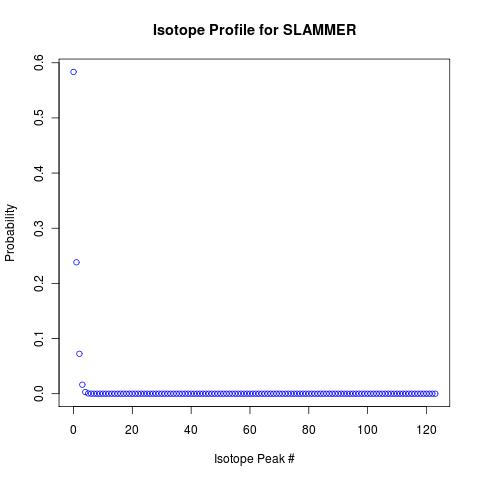
\includegraphics[scale=0.6]{isotope-profile.jpg}

As you can see, the values are pretty close for first isotope. But the values vary for subsequent isotopes. I attribute this to the errors accumulated during computation of FFT. The values of roots of unity might not be accurate enough to produce accurate results. The inaccuracy is not so evident in 0th isotope profile because it is obtained by multiplying $n$ elements for $n$ polynomials. But for an $i^{th}$ isotope, the probability value is obtained by multiplying many more numbers. Using some existing libraries like GNU-MultiPrecision library can definitely remove this problem. 

\subsection{Deuterium Exchange}
The isotope profile for this problem is obtained by reducing the number of hydrogens in SLAMMER by 60\% and rerunning the same program.  Here's the isotope profile for first ten values.

\ \\ \\ 

\begin{tabular}{|c|c|}
\hline
Isotope\# &  Mytool(\%) \\ \hline
0 & 58.64\\ \hline
1 & 27.90\\ \hline
2 & 9.84\\ \hline
3 & 2.50\\ \hline
4 & 0.53\\ \hline
5 & 0.1\\ \hline
6 & 0.01\\ \hline
7 & 0.00\\ \hline
8 & 0.00\\ \hline
9 & 0.00\\ \hline
\end{tabular}


The values for 0th, 1st, 2nd isotopes change significantly but the values for other isotopes almost remain almost same to the original SLAMMER profile. This is because abundance of H-2 is just 0.00015 when compared to other isotopes like S-33 that has .0421 abundance. Therefore, the effect of deuterium exchange is not profound on higher isotopes.

\section{Problem-2}
Inspect tool has many methods of evaluating the results. It uses p-values to rank each peptide found in the search. P-values tell the probability that the identified peptide is spurious. Thus lower the p-value, the better the results are. There are two methods for computing p-values. One is to search the spectra against a decoy database and generate false discovery rate and f-score. Then compute the p-value. Another method is to fit a mixuture model of emperical distributions of F-scores just like how PeptideProphet does.

There is also the MQScore metric which scores the actual match quality. 

DeltaScore measures the difference between MQScore for this match and the next best match. There is also DeltaScore-Other metric. Eventhough there are so many metrics, p-value is generally the widely used among them. 
 
Since Inspect's output is too verbose, I used the Summary.py file available with Inspect. I downloaded Inspect tool, compiled in my machine and ran Summary.py on my result set. The output gives identified peptides grouped by proteins. The top identification are the ones that have the lowest p-value and highest MQ-Scores for that peptide. 

\end{document}

